
\chapter{Calmodulin}
\label{chap:calmodulin}


\section{Calmodulin superfamily}

Calmodulin (CaM) was first discovered in 1963 in brain and heart.
Later on, it was found that CaM is a calcium-binding protein
(Sect.\ref{sec:calcium-binding-proteins}) with 4 EF-hand $\Ca$-binding motifs,
thus giving it the name Calmodulin ({\bf CALcium MODulated proteIN}, CaM), first
suggested by Cheung \citep{cheung1970, cheung1980}. 


The largest group of
Ca2+-binding proteins belongs to the calmodulin (CaM) superfamily. CaM
superfamily includes $\approx$ 600 proteins; with about 300 target proteins
whose conformational changes as the result of CaM binding.


\begin{mdframed}
Other names:
calcium-dependent regulator modulator protein, calcium-dependent regulator
(CDR), activate protein and troponin-C-like protein \citep{jurado1999la}.

\end{mdframed}



Calmodulin is a major calcium transducer and plays crucial role to the
metabolism and physiology of
eukaryotes\footnote{\url{http://www.ebi.ac.uk/interpro/potm/2003_3/Page_1.htm}}.
\footnote{\url{http://www.ebi.ac.uk/interpro/potm/2003_3/Page_1.htm}}.

\subsection{structures}

\begin{enumerate}
  \item  a pair of N-terminal (EF-hand 1 and EF-hand 2) and 
  
  \item C-terminal EF-hand (EF-hand 3 and EF-hand 4)
\end{enumerate}

\url{http://www.nostatic.com/proteins/calmodulin/CalmodStruc.htm}


\section{Calmodulin: apocalmodulin (ApoCaM), Ca2+-bound Calmodulin ($\Ca$-CaM)}
\label{sec:calmodulin_extension}
\label{sec:calmodulin}

Calmodulin's structure is very similar to the structure of troponin C (which is
another calcium binding protein). They are both members of the EF-hand
superfamily.

\begin{enumerate}
  \item  The presence of Ca2+/CaM is required for phosphorylation of several proteins
(myosin light chain kinase, phosphorylase kinase).

  \item CaM-kinase II mediates the secretion of neurotransmitters

It activates tyrosine hydroxylase required in catecholamine biosynthesis
NOTE: CaM-kinase II is capable of autophosphorylation even in the absence of
Ca++.
  
  \item  CaM regulates adenylate cyclase (cAMP), and cAMP regulates CaM. 
  
  \item A-kinase, regulated by CaM, phosphorylates the IP3 receptor
  
  \item  cAMP and CaM-kinases control CREB
  
  \item CaM activates cyclic nucleotide phosphodiesterase - an enzyme degrading
  cAMP. 
  
  \item 
\end{enumerate}

\subsection{-- distribution}

Calmodulin is ubiquitous and is found in many cell types, at various
subcellular locations (e.g. the cytoplasm, inside the organelles, or
associated with the plasma or organelle membranes).
\textcolor{red}{Calmodulin exists in 2 forms: Ca2+-free (apocalmodulin), and
Ca2+-bound.}

% CaM is ubiquitous and is found in many cell types, at various subcellular
% locations (e.g. the cytoplasm, inside the organelles, or associated with the
% plasma or organelle membranes). For more details, look at the book Heart
% Electrophysiology. 

\subsection{-- why Calcium-calmodulin?}

Calmodulin (CaM) is a small acidic (pI = 3.9-4.3), highly conserved 17kDa
protein (148 a.a in vertebrates) with high affinity for $\Ca$~\citep{Chin2000a}.

There are two globular domains in CaM, each containing a pair of
helix-loop-helix Ca2+-binding motifs called EF-hands, i.e. giving 4 EF-hand
$\Ca$-binding sites for each Calmodulin molecule,
Fig.\ref{fig:Calmodulin-4-EF-hands}. The EF-hand motif for calcium binding is
about 29 residues, consisting a 9-residue helix, followed by a 12-residue loop
and a 8-residue helix.

\begin{figure}[hbt]
  \centerline{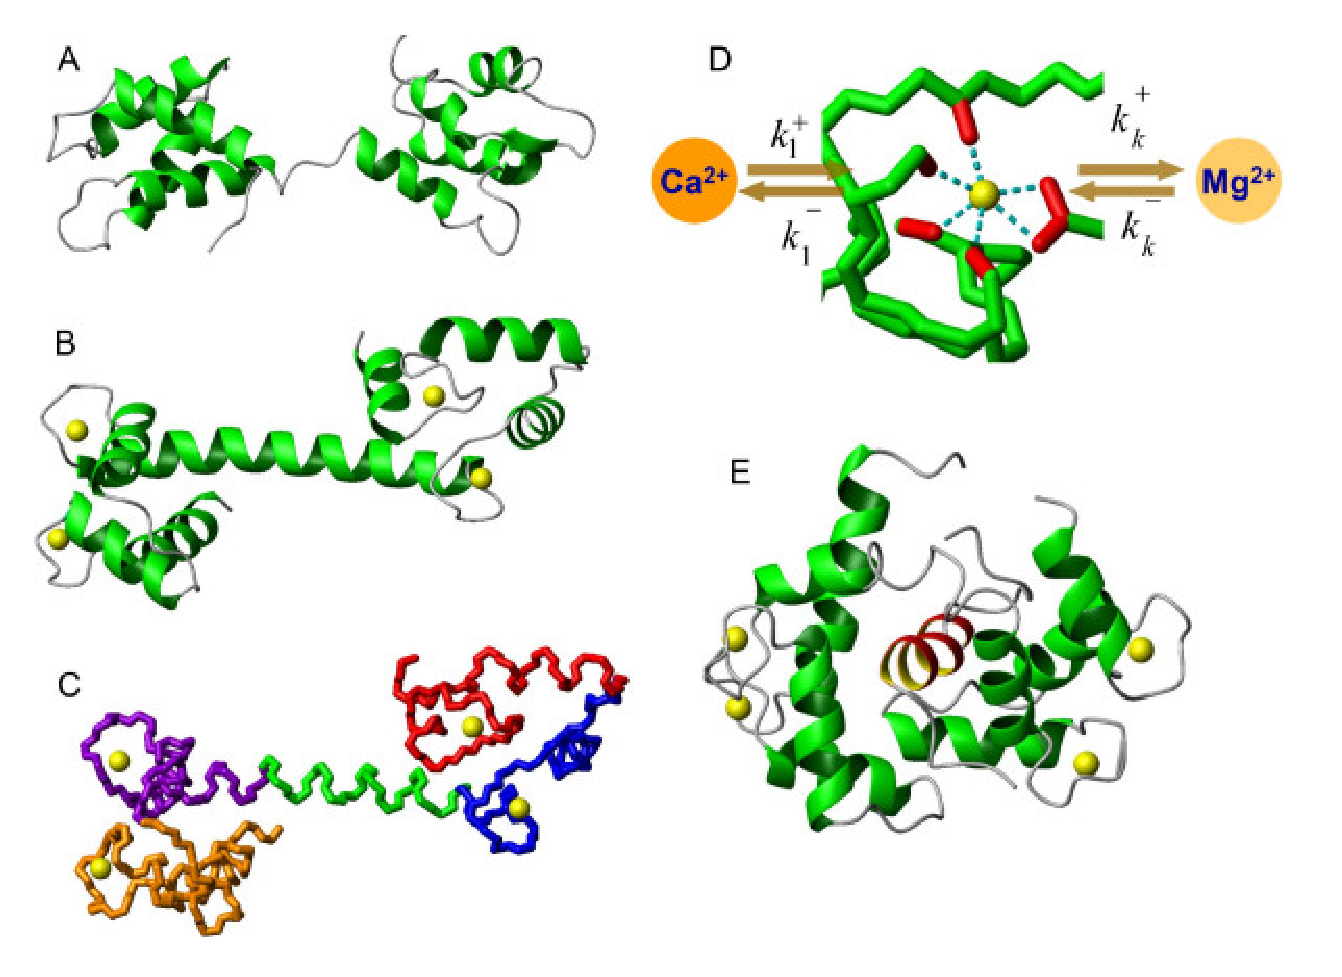
\includegraphics[height=6.6cm,
    angle=0]{./images/Calmodulin-4-EF-hands.eps}}
\caption{(A) $\Ca$-free Calmodulin vs. (B) $\Ca$-bound Calmodulin; (C) The
pairwise proximity of (red and blue, violet and brown) of four $\Ca$-binding EF
hand domains; (D) structure of the $\Ca$-loop on the N-terminal of CaM protein
- the dotted lines show interaction between $\Ca$ or $\Mg$ ion with Asp20,
Asp22, Asp24, Thr26, Glu31 residues; (E) Ribbon diagram showing $\Ca$/CaM
complex with the target peptide of protein kinase \citep{valeyev2008} }
\label{fig:Calmodulin-4-EF-hands}
\end{figure}


There are more than 500 known EF-hand proteins which are likely evolved from a
single EF-hand domain by duplication \citep{yang2003}. As calcium binding is
essential for the biological function of CaM, knowing the key determinants of
calcium binding affinity of CaM is important. The effectors can be calcium,
non-calcium ligand or protein environment. 

\subsection{-- how Ca2+/CaM complex work?}

$\Ca$ binding alters CaM conformation. Upon $\Ca$ binding, an activated
calmodulin changes its conformation which enable it to bind to a substrate, e.g.
a target protein and regulate the functions of that target protein, thereby
affecting many cellular functions (e.g. muscle contraction, short-term and
long-term memory, apoptosis - Sect.\ref{sec:apoptosis}, ...).
These target proteins (Sect.\ref{sec:cam-binding-proteins}) cannot bind calcium
directly, so they use calmodulin as a calcium-sensor and signal transducer
\citep{persechini1999}.


\begin{enumerate}
  \item  The best known canonical binding mode of CaM interaction with a
target is the "wrap-around" in which both N- and C-terminal domains of CaM bind
to the same target protein region, Fig.\ref{fig:Calmodulin-4-EF-hands}(E).

  \item A variation of the wrap-around CaM binding interaction has been shown to
  occur with the brain specific PKC substrate CAP-23/NAP-22 
  
  \item "extended" mode of interaction include anthrax exotoxin, Edema
  Factor, and Ca2+ Pump.

The extended mode of interaction is proposed to occur in target binding to
apo-CaM via the IQ motif.

  \item CaM-induced target dimerization has been reported as having another
  distinctly different binding mode. 

The dimerization of Ca2+-dependent K+ channels is achieved by adopting the
extended conformation of the EF-hand domains of CaM protein. Other examples of
target dimerization induced by CaM binding are the glutamate decarboxylase
(GAD) and transcription factor SEF2-1/E2-2.

\end{enumerate}

This suggests CaM interacts with phosphorylase kinase, CaATPase and skMLCK in
the apo state, but activates these proteins only when Ca2+ ions bind to a
CaM-target protein complex.

CaMKII kinase, on the other hand, binds to the Ca2+-CaM complex rather than
apo-CaM.

To elucidate the mechanisms underlying Ca2+/CaM-dependent target regulation,
researchers have measured the kinetics and steady-state levels of
CaM-target binding.

% In addition, the Calcium-Calmodulin complex is responsible for $\Ca$-dependent
% regulation of the activities of a vast array of different proteins (enzyme,
% pumps, and ionic channels\ldots) .
Target of Ca2+/CaM complex:
\begin{itemize}
  \item  \textcolor{red}{PMCA}: Sect.\ref{sec:PMCA}

Among those with high affinity (Kd = 5 nM) for the calmodulin-calcium complex
is the PMCA.
However, the free calmodulin-binding domain of the PMCA also interacts
with the ATP-binding site of the pump and acts as an inhibitor of ATP-driven pump
function

  \item IP3R - Sect.\ref{sec:IP3R-inhibition}
  
\end{itemize}
  

\subsection{-- affinity}

First, we need to know there are different mechanisms leading to
Ca2+/CaM-dependent target regulation. There are 4 $\Ca$ binding sites.

At normal condition, the binding affinity to $\Ca$ is $K_a = 1-10 \muM^{-1}$ at
low ionic strength \citep{linse1991}.
When local $\Ca$ increases to 5-20$\muM$, calcium then bind to CaM. Also, the
binding affinity is pH-dependent. The increase of pH raises affinity to Ca2+ and
eliminates cooperativity between Ca2+ binding sites on CaM \citep{valeyev2008}.

Because of its high binding capacity and affinity, Calmodulin plays an important
role in spatial propagation of calcium signals. 

\begin{enumerate}
  
  \item CaM-Ca complex has high affinity to PMCA: $K_d = 5$ (nM) -
  Sect.\ref{sec:PMCA-activator}.
  
  \item CaM bind all three RyR isoforms at nanomolar affinity irrespective RyR
  is Ca-free or Ca-bound. The stoichiometry is one CaM bind to one RyR subunit
  (Sect.\ref{sec:RyR-Ca2+-calmodulin}).
  
  \item At the physiological condition, calmodulin normally tethers with L-type calcium
channels, and when calcium ions bind to calmodulin, it triggers the inactivation
process to the associated L-type calcium channel -
Sect.\ref{sec:LCC_activation_inactivation}.
\end{enumerate}

Compared with TpnC, CaM has the similar primary, secondary and 3D structures
with an identical geometry of calcium binding pockets \citep{yang2002}. However,
its binding affinity differs by a magnitude of 3, and TpnC cannot activate most
of CaM's targets. Also, cardiac-Troponin C (cTpnC) has a higher affinity for
$\Ca$ in its C-terminal ($K_d=0.1\muM$), than CaM ($K_d=1-10\muM$)
\citep{george1993}.

CaM can also affect SR $\Ca$ release by acting on other proteins, e.g. DHPR,
CaMKII and calcineurin (a CaM-activated protein phosphatase).



\subsection{Ca2+-binding sites}

CaM can make use of the \ce{Ca^2+} from the SR or ER, besides using the calcium
influx from the extracellular environment when there is an action potential. 
% CaM can make use of \ce{Ca^2+} in the SR (sarcoplasmic reticulum) or
% ER (endoplasmic reticulum) and it can bind up to 4 \ce{Ca^2+}.

The maximum number of calcium ions binding to one calmodulin molecule is 4, i.e.
CaM has the 4 EF-Hand calcium-binding
motifs\footnote{\url{http://en.wikipedia.org/wiki/EF_hand}}.

Further, a CaM can undergo post-translation modifications (e.g.
phosphorylation, acetylation, methylation, proteolytic cleavage) which can
potentially modulate (enhance/down-regulate) its functions.


\section{CaM-binding proteins}
\label{sec:cam-binding-proteins}


\begin{figure}[htb]
  \centerline{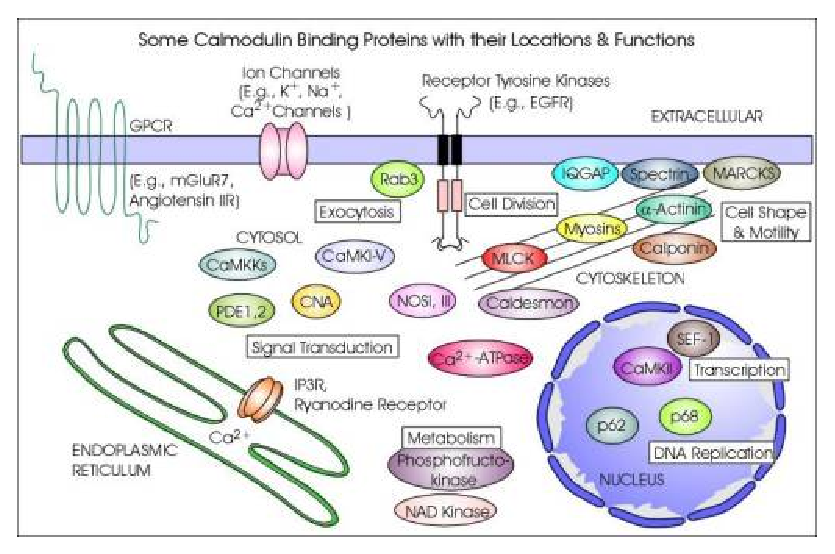
\includegraphics[height=7cm]{./images/CaM-binding-proteins.eps}}
  \caption{CaM-binding proteins}\label{fig:CaMBOT}
\end{figure}

CaM-binding proteins (CaMBP) is a diverse group of protein, as shown in
Fig.\ref{fig:CaMBOT}. There are more than 100 known target proteins to Ca2+/CaM,
e.g. protein kinases (like CaMKII), and phosphatases.

The binding and regulation by CaM can be categorized into 2 modes:
calcium-dependent (\ce{Ca^2+}-CaM) and calcium-independent (\ce{Ca^2+}-free or
{\it apocalmodulin} (ApoCaM)).

\textcolor{red}{\bf The question is how can CaM recognize which target protein
to bind to?} - The answer is there is no general models of target recognition.
In fact, there are several mechanism of interactions that have been described
for different targets.

\ce{Ca^2+}-CaM-binding proteins kinases, phosphatases, second
messenger signalling proteins, cytoskeletal and muscle proteins.
These proteins can be either \ce{Ca^2+}-activated or
\ce{Ca^2+}-inhibited.

\begin{enumerate}
  \item RyR - Sect.\ref{sec:calmodulin-RyR1}
\end{enumerate}


%%% Local Variables: 
%%% mode: latex
%%% TeX-master: "cardiology"
%%% End: 
